\documentclass[11pt]{article}
\usepackage{amsmath}
\usepackage{physics}
\usepackage{amssymb}
\usepackage{graphicx}
\usepackage{hyperref}
\usepackage{amsfonts}
\usepackage{cancel}
\usepackage{xcolor}
\hypersetup{
	colorlinks,
	linkcolor={black!50!black},
	citecolor={blue!50!black},
	urlcolor={blue!80!black}
}
\newcommand{\f}[2]{\frac{#1}{#2}}
\usepackage{newpxtext,newpxmath}
\usepackage[left=1in,right=1in,top=1.25in,bottom=1.25in]{geometry}
\usepackage{framed}
\usepackage{enumerate}

\usepackage{caption}
\usepackage{subcaption}

%\newcommand{\fig}[1]{figure #1}
%\newcommand{\explain}{appendix?}
%\newcommand{\rat}{\mathbb{Q}}
%
%\newcommand{\mathbb{R}}{\mathbb{R}}
%\newcommand{\nat}{\mathbb{N}}
%\newcommand{\inte}{\mathbb{Z}}
%\newcommand{\M}{{\cal{M}}}
%\newcommand{\sss}{{\cal{S}}}
%\newcommand{\rrr}{{\cal{R}}}
%\newcommand{\uu}{2pt}
%\newcommand{\vv}{\vec{v}}
%\newcommand{\comp}{\mathbb{C}}
%\newcommand{\field}{\mathbb{F}}
%\newcommand{\f}[1]{ \hspace{.1in} (#1) }
%\newcommand{\set}[2]{\mbox{$\left\{ \left. #1 \hspace{3pt}
%\right| #2 \hspace{3pt} \right\}$}}
%\newcommand{\integral}[2]{\int_{#1}^{#2}}
%\newcommand{\ba}{\hookrightarrow}
%\newcommand{\ep}{\varepsilon}
%\newcommand{\limit}{\operatornamewithlimits{limit}}
%\newcommand{\ddd}{.1in}
%\newcommand{\ccc}{2in}
%\newcommand{\aaa}{1.5in}
%\newcommand{\B}{{\cal B}}
%\newcommand{\C}{{\cal C}}
%\newcommand{\D}{{\cal D}}
%\newcommand{\FF}{{\cal F}}
\usepackage{amssymb}% http://ctan.org/pkg/amssymb
\usepackage{pifont}% http://ctan.org/pkg/pifont
\newcommand{\cmark}{\ding{51}}%
\newcommand{\xmark}{\ding{55}}%
\newcommand{\p}{\partial}%
%\usepackage{MnSymbol,wasysym}



\usepackage{listings}
\captionsetup[lstlisting]{margin=0cm,format=hang,font=small,format=plain,labelfont={bf,up},textfont={it}}
\renewcommand*{\lstlistingname}{Code \textcolor{violet}{\textsl{Mathematica}}}
\definecolor{gris245}{RGB}{245,245,245}
\definecolor{olive}{RGB}{50,140,50}
\definecolor{brun}{RGB}{175,100,80}
\lstset{
	tabsize=4,
	frame=single,
	language=mathematica,
	basicstyle=\scriptsize\ttfamily,
	keywordstyle=\color{black},
	backgroundcolor=\color{gris245},
	commentstyle=\color{gray},
	showstringspaces=false,
	emph={
		r1,
		r2,
		epsilon,epsilon_,
		Newton,Newton_
	},emphstyle={\color{olive}},
	emph={[2]
		L,
		CouleurCourbe,
		PotentielEffectif,
		IdCourbe,
		Courbe
	},emphstyle={[2]\color{blue}},
	emph={[3]r,r_,n,n_},emphstyle={[3]\color{magenta}}
}






\begin{document}
\begin{center}
{\large \bf PH312: Reflection \#9}\\
{ Huan Q. Bui}\\
April 22, 2021
\end{center}

While I've seen the Bernoulli's principle before and how it is usually used to explain lift and flight, I never realized that it is not enough and that Bernoulli's principle alone would lead to a circular argument. This was eye-opening.\\


I am also surprised to see that boundary layers are a big deal. I think from what we've seen so far, all the cool fluid dynamical phenomena are due to boundary-layer effects. The vortex loop created by a 3d foil was very amusing. I have always imagined vortices due to the wing tip as two separate vortex tubes and had no idea that they are actually one connected tube.\\


I play ultimate frisbee at Colby as a handler (equivalent of quarter-back/thrower in American football), so our discussion of how drag due to circulation due to spin may induce swirls and other beautiful disc trajectories really resonates with me. The discussion also lets me appreciate the very clever engineering of the frisbee.

\begin{figure}[!htb]
	\centering
	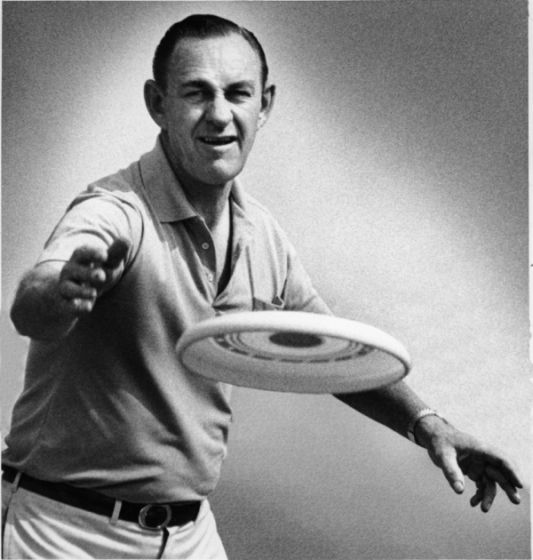
\includegraphics[scale=0.5]{fris}
\end{figure} 

The frisbee isn't simply an ordinary disc, is it? Its inward-curving edge allows it to always be a ``wing'' while spinning, and so that when it is thrown, there is vertical lift as well as other forces due to the direction of spin and angle of release. It's also fascinating that I (or anybody who practices throwing frisbees a lot) just \textit{intuitive understand} all the parameters  controlling the frisbee's flight and am able to make the disc fly in whatever trajectory I want without any real understanding of the fluid mechanics behind each throwing technique.



\end{document}




